%%%%%%%%%%%%%%%%%%%%%%%%%%%%%%%%%%%%%%%%%
% Simple Sectioned Essay Template
% LaTeX Template
%
% This template has been downloaded from:
% http://www.latextemplates.com
%
% Note:
% The \lipsum[#] commands throughout this template generate dummy text
% to fill the template out. These commands should all be removed when 
% writing essay content.
%
%%%%%%%%%%%%%%%%%%%%%%%%%%%%%%%%%%%%%%%%%

%----------------------------------------------------------------------------------------
%	PACKAGES AND OTHER DOCUMENT CONFIGURATIONS
%----------------------------------------------------------------------------------------

\documentclass[12pt]{article} % Default font size is 12pt, it can be changed here

\usepackage[margin=1in]{geometry} % Required to change the page size to A4
\geometry{a4paper} % Set the page size to be A4 as opposed to the default US Letter

\usepackage{graphicx} % Required for including pictures

\usepackage{float} % Allows putting an [H] in \begin{figure} to specify the exact location of the figure
\usepackage{wrapfig} % Allows in-line images such as the example fish picture

\usepackage{lipsum} % Used for inserting dummy 'Lorem ipsum' text into the template

\usepackage{hyperref}
%\usepackage{apacite}
\usepackage{tikz}

\linespread{1} % Line spacing

%\setlength\parindent{0pt} % Uncomment to remove all indentation from paragraphs

\usepackage{soul} %for \hl to highlight
%\usepackage[final,inline,nomargin]{fixme}
\usepackage[draft,inline,nomargin]{fixme}
\newcommand{\hlfixme}[1]{\fxfatal{\hl{#1}}}
\newcommand{\hlfxnote}[1]{\fxnote{\hl{#1}}}

\graphicspath{{Pictures/}} % Specifies the directory where pictures are stored

\bibliographystyle{abbrv}

\begin{document}

%----------------------------------------------------------------------------------------
%	TITLE PAGE
%----------------------------------------------------------------------------------------

\begin{titlepage}

\newcommand{\HRule}{\rule{\linewidth}{0.5mm}} % Defines a new command for the horizontal lines, change thickness here

\center % Center everything on the page

\textsc{\LARGE New York University}\\[1.5cm] % Name of your university/college
\textsc{\Large Big Data: Critical Perspectives}\\[0.5cm] % Major heading such as course name
\textsc{\large Project Proposal}\\[0.5cm] % Minor heading such as course title

\HRule \\[0.4cm]
{ \huge \bfseries Predictive Policing - Opaqueness, Impact and Legal Standards}\\[0.4cm] % Title of your document
\HRule \\[1.5cm]

\begin{minipage}{0.4\textwidth}
\begin{flushleft} \large
\emph{Author:}\\
Kevin \textsc{Gallagher} % Your name
\end{flushleft}
\end{minipage}
~
\begin{minipage}{0.4\textwidth}
\begin{flushright} \large
\emph{Professor:} \\
Helen \textsc{Nissenbaum} % Supervisor's Name
\end{flushright}
\end{minipage}\\[4cm]

{\large \today}\\[3cm] % Date, change the \today to a set date if you want to be precise

%\includegraphics{Logo}\\[1cm] % Include a department/university logo - this will require the graphicx package

\vfill % Fill the rest of the page with whitespace

\end{titlepage}

%----------------------------------------------------------------------------------------
%	TABLE OF CONTENTS
%----------------------------------------------------------------------------------------
\clearpage\thispagestyle{empty}\addtocounter{page}{-1}
\tableofcontents % Include a table of contents
\newpage % Begins the essay on a new page instead of on the same page as the table of contents 

%----------------------------------------------------------------------------------------
%	INTRODUCTION
%----------------------------------------------------------------------------------------

\begin{abstract}
The abstract will go here.
\end{abstract}
\newpage
\section{Introduction}\label{sec:introduction} % Major section

One Friday morning in July of 2011, two women were arrested in Santa Cruz, California after being caught peering into cars parked in a local parking garage. In addition to the suspicious nature of their activities, one of the women arrested had outstanding warrants, and the other was in possession of drugs. Though arrests of this nature are rarely reported on the news, this particular arrest was an exception due to its peculiar circumstances. These arrests were made after officers were dispatched beause a computer algorithm predicted the area as likely to be effected be crime. \cite{nyt} 
This technology, called Predictive Policing, is definied as the application of analytical techniques, particularly quantitative techniques, to identify promising targets for police intervention and prevent or solve crime. \cite{perryetal} As such, predictive policing can be seen as a branch of ``Big Data'' or ``Data Science,'' the collection and analysis of large quantities of data to form predictive tools.

The purpose of this paper is to analyze the effect of predictive policing on due process. To achieve this, the effects of predictive policing will be viewed through a multidisciplinary eye. Legal literature will be reviewed to define and discuss the role of due process in liberal democracies, psychology literature will be reviewed to discuss conceptual models of thinking and computer science literature will be discussed to discuss the inner workings of machine learning. In order to tie all of these different disciplines together, this paper discusses all of them through the lense of probability and liklihood.

The remainer of this paper will be organized as follows, Section \ref{subsec:predictivepolicing} will define predictive policing.
% and give a brief outline of the current relevant literature.
Section \ref{subsec:dueprocess} will define due process and discuss its role in liberal democracies. Section \ref{subsec:machinelearning} will discuss machine learning and probability and their roles in predictive policing. Section \ref{subsec:cognitive} will introduce elements of cognitive psychology. Section \ref{sec:oldvnew} will discuss the changes to due process introduced by predictive policing. Finally, Section \ref{sec:conclusion} concludes.

%\hlfixme{Some metrics. Not 100\% sure what this means. Talk to Helen about it.}
%------------------------------------------------
\subsection{Predictive Policing: Definition and Taxonomy} \label{subsec:predictivepolicing}% Sub-section

As mentioned in Section \ref{sec:introduction}, predictive policing is by Perry et al. to be the application of analytical techniques, particularly quantitative techniques, to identify promising targets for police intervention and prevent or solve crime. In the book \textit{Predictive Policing: The role of crime forcasting in law enforcement operations}, Perry et al. present a taxonomy of predictive policing methods. This taxonomy breaks predictive policing into four categories: \cite{perryetal}

\begin{enumerate}
\item Methods for predicting future crimes
\item Methods for predicting future offenders
\item Methods for predicting perpetrator's identities
\item Methods for predicting victims of crimes
\end{enumerate}

Category one, methods for predicting future crimes, focuses on predicting the times and places in which crimes are anticipated to occur. Category two, methods for predicting future offenders, focuses on predicting individuals and groups that are ``at risk of offending in the future.'' Category three, methods for predicting perpetrator's identities, focuses on identifying individuals who have committed past crimes. Lastly category four, methods for predicting victims of crimes, focuses on predicting individuals and groups that are ``likely to become victims of crime.''

%------------------------------------------------
%
% DELETED CONTENT
%
%------------------------------------------------
%The questions raised by these categories of predictive policing will be addressed seperately as to follow the layout of the taxonomy.
%------------------------------------------------
%
% END OF DELETED CONTENT
%
%------------------------------------------------

\subsection{Due Process} \label{subsec:dueprocess}
%\hlfixme{Introduce the ideas of due process here, and why they are important. Inclue defition from OED and do a quick lit review. Maybe ask Jessica.}
Due Process is defined by the Oxford English Dictionary (US Edition) to be ``[f]air treatment through the normal judicial system, especially as a citizen’s entitlement.'' In modern liberal democracies (such as the United States), due process serves an important role; Due process protects citizens from unfair treatment under the law. 

Liberal democracies have at the core of their philosophies the idea that every individual has equal protection of human rights, civil rights, civil liberties, and other political freedoms. As such, due process of law is necessary to protect the core tenants of this philosophy, and to protect the rights of citizens from governments that seek to violate the rights of its citizens. It ensures that the weak, poor and powerless have the same legal protections as the strong, wealthy and powerful, creating equal treatment under the law.

In the United States, due process of law is seperated into two groups, proceedural due process and substantive due process. Procedural due process focuses on rights that apply to government proceedings that may result in the denial of an individual's right to life, liberty or property \cite{wex_procedural}. As part of procedural due process, it is well accepted that the following rights apply: \cite{friendly}

\begin{enumerate}
\item An unbiased tribunal.
\item Notice of the proposed action and the grounds asserted for it.
\item Opportunity to present reasons why the proposed action should not be taken.
\item The right to present evidence, including the right to call witnesses.
\item The right to know opposing evidence.
\item The right to cross-examine adverse witnesses.
\item A decision based exclusively on the evidence presented.
\item Opportunity to be represented by counsel.
\item Requirement that the tribunal prepare a record of the evidence presented.
\item Requirement that the tribunal prepare written findings of fact and reasons for its decision.
\end{enumerate}

Substantive due process is ``[a] doctrine holding that the 5th and 14th Amendments require all governmental intrusions into fundamental rights and liberties be fair and reasonable and in furtherance of a legitimate governmental interest.'' \cite{wex_substantive} One part of substantive due process is the application of the Bill of Rights, which contains as part of it the Fourth Amendment, or the protection against unreasonable searches and seizures by the government.

In modern policing, two legal standards keep the actions of law enforcement agencies in check: reasonable suspicion and probable cause. Reasonable suspicion is the standard that must be met in order for law enforcement officials to justify brief stops and detentions, but not full searches. \cite{wex_suspicion} Reasonable suspicion must be based on ``specific and articulable facts... taken together with rational inferences from those facts,'' which must be associated with a particular individual. \cite{terry} In order to receive a warrant for a search or to make an arrest, a law enforcement agent must meet the standard of probable cause. Probable cause requires a ``reasonable basis for believing that a crime may have been committed (for an arrest) or when evidence of the crime is present in the place to be searched (for a search).'' \cite{wex_cause} These standards keep the police from arbitrarily targeting individuals for investigation of crimes, instead requiring reasons for the infringement on their rights.

\begin{figure}
\begin{center}
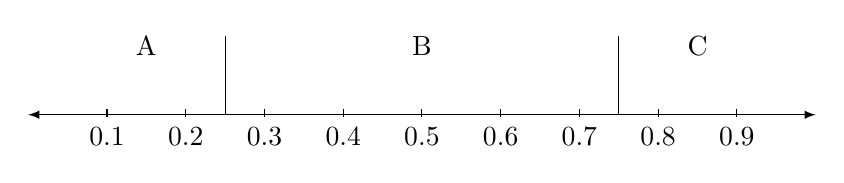
\begin{tikzpicture}
% a straight line segment
\draw[latex-latex] (0,0) -- (10,0);
% the ticks and their labels
\foreach \x  in {0.1,0.2,0.3,0.4,0.5,0.6,0.7,0.8,0.9}
  \draw[xshift=\x*10 cm] (0pt,2pt) -- (0pt,-1pt) node[below,fill=white] {\the\numexpr\x};
% the thicker segment
%\draw[ultra thick] (2.06,0) -- (8.94,0);
% the labels
%\node[fill=white,draw=black,circle,inner sep=2pt,label=above:{$p_1=.25$}] at (2.5,0) {};
%\node[fill=white,draw=black,circle,inner sep=2pt,label=above:{$p_2=.75$}] at (7.5,0) {};
%\node[fill=black,draw=black,circle,inner sep=2pt, label=below:{0} at (0,0) {};
%\node[fill=black,draw=black,circle,inner sep=2pt, label=below:{1} at (10,0) {};
%\node at (5.5,-0.8) {$\mu$};
\draw (2.5,0) -- (2.5,1);
\draw (7.5,0) -- (7.5,1);
\node [label=above:{A}] at (1.5,0.5) {};
\node [label=above:{B}] at (5,0.5) {};
\node [label=above:{C}] at (8.5,0.5) {};
\end{tikzpicture}
\caption{The number line seperated into three sections by $p_1$ and $p_2$.}
\label{fig:numberline}
\end{center}
\end{figure}

To frame this into the discussion of probabilities, we can think of redefining reasonable suspicion and probable cause as probability threshold values $p_1$ and $p_2$ respectively, where $0 < p_1 < p_2 < 1$, where the values of $p_1$ and $p_2$ are defined by societal norms, legislation and case law. (Picking these values is not trivial, though the abstraction is still useful; we will not discuss the values of $p_1$ or $p_2$ in this paper.) These values divide a number line on the interval [0,1] into three parts, as shown (with example values of $p_1$ and $p_2$ in Figure \ref{fig:numberline}. If the perceived probability $P$ (we will define this term contextually in both Sections \ref{subsec:cognitive} and \ref{subsec:machinelearning}) is greater than $p_1$, but less than $p_2$, (i.e. $p_2 \geq P > p_1$), only the standard of reasonable suspicion is met. This can be seen as section B of the numberline. If the perceived probability is above $p_2$ (i.e. $P > p_2$), the standards of probable cause and reasonable suspicion are met. This can be seen as section C of the number line. This reflects the fact that reasonable suspicion is a lesser standard than probable cause. If the perceived probability is less than $p_1$ (i.e. $P \leq p_1$), neither probable cause nor reasonable suspicion are met. This corresponds to section A of the number line. Though this numerical definition of these two standards may seem overly complex, they are necessary to tie together the disciplines of law, psychology and computer science.

\subsection{Cognitive Psychology} \label{subsec:cognitive}
In order to understand judgements made by police before the creation of predictive policing, one must understand how to mind deals with decisions of a statistical nature. These ideas are detailed greatly by the work of Kahneman and Tversky, two psychologists who created and studied a useful model of human statistical thinking. This section briefly outlines the work done by Kahneman and Tversky in this field and is based entirely on Khaneman's book \textit{Thinking Fast and Slow}.\cite{kahneman}

In \textit{Thinking Fast and Slow}, Kahenman describes his work with Tversky in different areas of psychology. The central thesis of the book, and of Kahenman and Tversky's work itself, is the idea of a human's thought process being seperated into two modes of thought, called ``system 1 and system 2'' both in the academic literature and in the book itself. In the book, Kahneman explains that system 1 is fast and effortless. It acts as a statistician, counting occurences and making quick predictions and reactions based on input stimuli. As such, it is trained over many years of input data and outcomes, calculating correlations and storing them for later use. System 1 is also responsible for expert reactions to domain specific problems. System 2 is the antithisis of system 1. It is slow, effortful and logical, and it analyzes new problems and stimuli that system 1 was incapable of handling, or was proven to have handled incorrectly. Due to the effortful nature of system 2, most decisions, predictions, judgements and reactions are made by system 1, the quick and intuitive mode of thinking. In order to avoid activating the slow and effortful system 2, there exist a list of heuristics that allow individuals to reach decisions using only system 1, including framing, availability, loss aversion, and others.

Since system 1 is responsible for quick expert decisions, it is reasonable to believe that when a law enforcement agent attempts to assess whether a standard of probable cause or reasonable suspicion are met, they use the quick and intuitive ``statistician'' that is system one. To place this in context of our frame of probability, this can be viewed as a law enforcement agent estimates the perceived probability $P = f(x_1,...,x_n)$, that is the probability that an observed individual has committed or is going to commit a crime. This probability is estimated based on expert training (police training) and previous similar experiences. Then, the law enforcement agent estimates the values of $p_1$ and $p_2$ based on his or her understanding of the legislation and case law. Lastly, he or she compares the perceived probabilty $P$ with the thresholds $p_1$ and $p_2$ as described in Section \ref{subsec:dueprocess}.

%------------------------------------------------

%\subsection{Subsection 2} % Sub-section



%------------------------------------------------

%\subsubsection{Subsubsection 1} % Sub-sub-section



%------------------------------------------------

%\subsubsection{Subsubsection 2} % Sub-sub-section



%----------------------------------------------------------------------------------------
%	MAJOR SECTION 1
%----------------------------------------------------------------------------------------

\section{The Novelty of Predictive Policing}\label{sec:oldvsnew} % Major section
%As previously mentioned, predictive policing is an extention of big data into the field of policing and law enforcement. As such, it inherits many of the problems that big data exhitbits, such as a lack of transparency and issues of bias. In addition to these issues, the application of big data to the realm of policing creates whole new questions, such as the question of how effectiveness is measured, and what role probability and statistics plays in the standards of due process, such as reasonable suspicion and probable cause. In addition, mistakes in law enforcement action taken in response to the predictions made carry potentially high costs to law enforcement and private citizens alike. In this section, these issues will be explored and addressed, and will be tied back to the cases mentioned in Section \ref{sec:introduction}.

\subsection{Similarities} \label{subsec:Similarities}
%One historical problem that big data struggles with is the problem of transparency. In many realms in which big data is used, such as credit reporting, advertising, data brokers, employment, housing and others, decisions made based on prediction algorithms affect the lives of countless individuals. However, due to claims of intellectual property and trade secrests individuals have no ability to peer into the machines that dictate the directions of certain aspects of their lives. Worse, even when individuals are not blocked by legal and business challenges, often times peering into an algorithm does nothing to help an individual to understand why a particular classification was made. Part of this lies in the fact that the prediction algorithms are hard to understand by a layperson, but part of it also lies in the technology itself. 

%One large part of the big data aparatus is the application of machine learning, or an area of statistics and computer science in which computers determine correlations between input features and predicted labels. %TODO ADD AN EXAMPLE.
%One of the great strengths of machine learning is to find correlations that human experts cannot. This is done by the pure computational power that a machine possesses and people do not. However, this strength is also a great weakness. Due to the fact that a machine can predict based on input patterns that may escape a human expert, a large amount of opacity enters the system, even when the engineers and statisticians themselves are involved. Even if a domain expert is able to determine why a prediction algorithm output a certain prediction, this solution is not scalable. The entire purpose of big data is to deal with quantities of data that are impossible for human teams to sift through, making it difficult for companies and agencies that employ big data techniquest to verify the accuracy and fairness of a prediction or classification.

%This opaquness poses a unique challenge for law enforcement purposes. As seen in the breakdown of procedural due process mentioned above, the justice system of liberal democracies requires a large amount of transparency. Individuals who have had an action taken against them must be able to defend themselves, and as such they need to know the reasons that lead to a particular action being taken. As predictive policing features more prominently in our justice system, it will begin to affect more and more police actions. As such, the police will need to be able to justify their actions and provide individuals with the evidence that was collected that allowed the police to do so. However, due to the opaque nature of big data such disclosures will be exceedingly difficult, if not impossible. This leads one to ask how much, if at all, should opaque big data classifications be used to guide police actions? By the breakdown of procedural due process given above, it would seem that the lack of transparency in predictive policing methods may threaten the liberties of an accused individual, and may even place the justification of law enforcement's actions into question.

\subsection{Differences}\label{subsec:differences}

%Until the era of big data began, actions taken by police were based on specific facts and tips provided by the circumstances of the crime or by witnesses of the crime the law enforcement agents were investigating. Because of this, police were able to articulate specific facts and circumstances that lead to the reasonable suspicion for brief stops or detentions and probable cause in order to obtain a warrant. However, the current use of big data challenges these well established standards and overall due process. This paper will attempt to address how big data and predictive policing change due process and the standards of reasonable suspicion and probable cause. 

%Another historical problem of big data is the introduction of biases. Though many proponents of big data claim that the introduction of statistical algorithms leaves little to no room for human bias, this is simply not the case.\cite{hardt} As mentioned previously, machine learning, which finds the correlations between inputs and classification labels, plays a large role in the aparatus of big data. Machine learning is split into the following phases:

%\begin{enumerate}
%\item Data collection.
%\item Feature creation.
%\item Feature selection and/or extraction.
%\item Data labeling.
%\item Algorithm training.
%\item Algorithm testing and validation.
%\item Production and classification.
%\end{enumerate}

%Though many proponents claim that raw data is discovered and fed into the algorithm, the steps above show that data goes through a lot of processing and transformation before the classification step is reached. As shown in step 2, human intervention is usually need to decide what aspects of the data become features. Though domain experts are usually consulted in this step, this interaction has the capability to introduce a large amount of human bias. For example, in Perry's report on predictive policing \cite{perryetal}, the idea of using quantitative measures such as the LSI-R in predictive policing algorithms is discussed. Though this could be seen as a positive step to introduce quantitative measures into the predictive policing, there are examples of bias even in the LSI-R. For example, in the South Dekota Department of Human Services LSI-R training slides, one of the included predictors of future crime is ``belonging to some minority groups.'' \cite{dekota} If the LSI-R scoring is based on racial bias, and the LSI-R numerical output is included as a feature in predictive policing, the output of the policing algorithm is at least in part based on the race of the individual, which is commonly accepted as wrong and unjust.  %TODO cite raw data is an oxymoron.

%In addition to being introduced at the feature creation and selection/extraciton phases, bias can also be introduced at the label phase. As shown in the series of steps above, machine learning algorithms must be trained. In many cases, supervised training algorithms are used, meaning that many instances of data and the ``correct'' output label are fed to the learning algorithm and a classification model is built based on this data. These labels, however, are not ``discovered.'' They are frequently assigned by domain experts and heuristic methods. This is another area in which human bias can find its way into big data.

%Claims of unbiased accuracy by proponents of big data, mixed with the lack of transparency that comes hand-in-hand with the technology, makes this a dangerous tool for use by law enforcement officials.

%\textbf{NOTE: In the remainder of this section I will tie in these issues with predictive policing and due process.}
%------------------------------------------------
%
% DELETED CONTENT
%
%------------------------------------------------
%Though predictive policing, in many ways, is simply a technological extention of work already done by police officers and other law enforcement officials (such as identifying hot spots and high profile repeat offenders)\cite{perryetal}, the automation of these processes introduce many questions. In particular, this paper proposes research into the four areas listed below that are affected by predictive policing.

%\begin{enumerate}
%\item \textbf{Opaqueness and Freedom of Information:} To what extent are the operations of these technologies understood by the departments who are using them? To what extent are they understood by the general public?
%\item \textbf{Fairness and Civil Liberties:} To what extent do the inputs of the classification or regression algorithms reflect social, economical and racial biases that currently exist? How does this affect minoirty groups? 
%\item \textbf{Impact:} How effective is predictive policing? How is its effectiveness measured, and why? Do these measurements make sense?
%\item \textbf{Due Process and Legal Standards:} In what ways does predictive policing change our understanding of current standards such as reasonable suspicion or probable cause? What affect will these have on individuals within communities utilizing these technologies? Who is held accountable for harms created by such algorithms?
%\end{enumerate}

%All of these questions are interrelated, as the accuracy, impact, fairness and opaqueness of predictive policing will likely affect the impact it has on due process and current legal standards. 

%This paper will draw on many related works published on predictive policing, including the Rand Corporation report written by Perry et al. \cite{perryetal}, which presents a definition of taxonomy of preictive policing, discusses the technical means through which predictive policing is performed, and provides advice to law enforcement personel with regards to how to technology is meant to be used. In addition, this work will draw on work presented in the article \emph{Data Derivatives On the Emergence of a Security Risk Calculus for Our Times} written by Louise Amoore \cite{amoore2011data}, which analyzes the derivation of risk scores for the purpose of national security. More, this work will draw on work presented in the 2010 National Research Council report entitled \emph{Protecting Individual Privacy in the Struggle Against Terrorists: a Framework for Program Assessment} written by Perry and Vest \cite{perryprotecting}, which analyzes and discusses the balance between national security and civil liberties, including privacy. This work will also draw on work done by Andrew Guthrie Ferguson which details possible effects of predictive policing on the standard of reasonable suspicion. \cite{ferguson2012predictive} Lastly, this work will also draw on various news articles, technical blog posts and other books and articles on the subjects of predictive policing, machine learning,data mining, and national security. \cite{hildebrandt2013privacy} \cite{hardt} \cite{robinson2014civil} \cite{intercept}

%In addition, this work will also attempt to obtain information about current practices, technological state of the art and other related topics from law enforcement agencies, attorneys, civil rights groups and other individuals and organizations familiar with the topic of predictive policing.\cite{dekota}

%------------------------------------------------
%
% END OF DELETED CONTENT
%
%------------------------------------------------


\section{Verdict and Conclusion}\label{sec:conclusion}
%This paper has analyzed and discussed the application of predictive policing and its effect on the realm of due process. As part of this, it has discussed what predictive policing is and how it is used, what due process is and why it is important in liberal democracies, and finally the drawbacks of big data and predictive policing, and how these drawbacks effect due process.

\nocite{*}
%------------------------------------------------

%\subsection{Subsection 1} % Sub-section

%\subsubsection{Subsubsection 1} % Sub-sub-section



%------------------------------------------------

%\subsubsection{Subsubsection 2} % Sub-sub-section



%------------------------------------------------

%\subsubsection{Subsubsection 3} % Sub-sub-section


%----------------------------------------------------------------------------------------
%	MAJOR SECTION X - TEMPLATE - UNCOMMENT AND FILL IN
%----------------------------------------------------------------------------------------

%\section{Content Section}

%\subsection{Subsection 1} % Sub-section

% Content

%------------------------------------------------

%\subsection{Subsection 2} % Sub-section

% Content

%----------------------------------------------------------------------------------------
%	CONCLUSION
%----------------------------------------------------------------------------------------

%\section{Conclusion} % Major section


%----------------------------------------------------------------------------------------
%	BIBLIOGRAPHY
%----------------------------------------------------------------------------------------
\newpage
\bibliography{references}


%----------------------------------------------------------------------------------------

%\newpage
%\center{\huge{NOTES}}
%\begin{itemize}
%\item Metrics - how to measure?
%\item Schultz and Crawford - definitions
%\item Why due process is important in a liberal democracy - Look at this
%\item Incursions of data science into the methodologies and procedures and how they may challenge the meaning/foundation of these.
%\item Need to fix and find citations
%\end{itemize}
\end{document}